% =====================================================================
% AURA — Final Tasarım Raporu (FTR) — GÖNDERİLECEK SÜRÜM
% Derleme:  xelatex FTR_GONDERILECEK.tex   (TOC için iki kez çalıştırın)
% Önce:     python tools/make_ftr_figures.py   (docs/figures/*.png üretir)
% Format: Arial 12 / başlık 14 bold / 1.15 satır / iki yana yaslı /
%         kenar üst 2.8 cm, diğer 2.5 cm / Kapak + İçindekiler ayrı sayfa.
% Sayılar GERÇEK ölçümlerden (eval_results/, weights/custom_*_s.metrics.json).
% =====================================================================
\documentclass[12pt,a4paper]{article}
\usepackage{fontspec}
\setmainfont{Arial}
\usepackage[a4paper,top=2.8cm,bottom=2.5cm,left=2.5cm,right=2.5cm]{geometry}
\usepackage{graphicx}
\graphicspath{{docs/figures/}}
\usepackage{booktabs}
\usepackage{tabularx}
\usepackage{array}
\usepackage{float}
\usepackage{setspace}
\setstretch{1.15}
\usepackage{xcolor}
\definecolor{aura}{HTML}{1b5e20}
\definecolor{aurab}{HTML}{0d47a1}
\usepackage{titlesec}
\titleformat{\section}{\fontsize{14}{16}\bfseries\color{aura}}{\thesection.}{0.5em}{}
\titleformat{\subsection}{\fontsize{12}{14}\bfseries\color{aurab}}{\thesubsection}{0.5em}{}
\titlespacing{\section}{0pt}{10pt}{4pt}
\titlespacing{\subsection}{0pt}{6pt}{2pt}
\usepackage[hidelinks]{hyperref}
\usepackage{caption}
\captionsetup{font=small,labelfont=bf,skip=3pt}
\captionsetup[figure]{name=Şekil}
\captionsetup[table]{name=Tablo}
\setlength{\parindent}{0pt}
\setlength{\parskip}{0.5pt}
\setlength{\emergencystretch}{3em}
\newcommand{\tcode}[1]{\texttt{\small #1}}

\begin{document}

% ========================= KAPAK (ayrı sayfa) =========================
\thispagestyle{empty}
\begin{center}
\vspace*{1.2cm}
{\fontsize{12}{14}\bfseries TEKNOFEST 2026}\\[2pt]
{\fontsize{12}{14}\selectfont 5G ve Yapay Zekâ ile Akıllı Yol Güvenliği Yarışması}\\[2.4cm]

{\fontsize{42}{46}\bfseries\color{aura} AURA}\\[3pt]
{\color{aura}\rule{0.5\textwidth}{1.2pt}}\\[12pt]
{\fontsize{15}{19}\bfseries 5G ve Yapay Zekâ ile Akıllı Yol Güvenliği Sistemi}\\[16pt]
{\fontsize{17}{21}\bfseries\color{aurab} FİNAL TASARIM RAPORU}\\[2.6cm]

\begin{tabular}{rl}
\textbf{Takım Adı:} & {\large\bfseries\color{aura}Nankatsu} \\[12pt]
\textbf{Takım ID:} & \underline{\hspace{5.2cm}} \\[12pt]
\textbf{Başvuru ID:} & \underline{\hspace{5.2cm}} \\[12pt]
\textbf{Tarih:} & 28.06.2026 \\
\end{tabular}

\vfill
{\small Bu rapordaki tüm başarım sayıları, gerçek test videoları ve ayrılmış (held-out) doğrulama
setleri üzerinde otomatik ölçüm hattıyla elde edilmiştir; yöntem ve sonuçlar Bölüm~4'te belgelenmiştir.}
\end{center}
\newpage

% ===================== İÇİNDEKİLER (ayrı sayfa) =======================
\thispagestyle{empty}
\renewcommand{\contentsname}{İçindekiler}
\tableofcontents
\newpage

% ============================ 1. ÖZET =================================
\section{Proje Özeti}
AURA, yol kenarı trafik kamerası akışından \textbf{araç, plaka, hız ve riskli sürücü
davranışı} tespiti yapan gerçek bir yapay zekâ çekirdeğini; bu çekirdeği \textbf{5G CAMARA
Quality-on-Demand (QoD)} ve \textbf{Number Verification (NV; sürücü telefon numarasının
operatör nezdinde sessiz doğrulanması)} telekom yetenekleriyle birleştiren uçtan uca bir sistemdir. Amaç, yol güvenliğini tehdit eden olayları (dikkatsiz sürüş, araç-içi
telefon/sigara kullanımı, hız ihlali) gerçek-zamanlıya yakın gecikmeyle tespit etmek ve \textbf{yalnızca
kritik anlarda} 5G şebeke kalitesini talep ederek bant genişliğini verimli kullanmaktır.

Proje kapsamında yürütülen başlıca faaliyetler: (i) YOLO26 tabanlı çok-aşamalı bir tespit/takip
hattının tasarımı; (ii) sürücü davranışı için landmark kütüphanesi gerektirmeyen, poz-geometrisi
ve nesne kanıtını birleştiren hibrit bir motor; (iii) Türk plaka formatına özgü, koruyucu karar
kurallarıyla donatılmış bir plaka okuma konsensüs döngüsü; (iv) CAMARA QoD ve NV sözleşmelerini
birebir taklit eden mock servisler; (v) çözümün üç gerçek test videosu ve held-out doğrulama
setleri üzerinde nicel sınanması. Yapay zekâ çekirdeği (tespit, takip, kararlılık, OCR, hız,
risk) \textbf{gerçektir}; telekom katmanları gerçek API sözleşmesini taklit eden \textbf{mock}'lardır
— gerçek operatöre geçişte uç nokta/kimlik değişir, ayrıca saha doğrulaması gerekir. Kalite güvencesi
olarak ${\sim}780$ birim/perf testi, statik denetim (\tcode{ruff}+\tcode{black}) ve otomatik
sürekli-entegrasyon hattı mevcuttur. İstatistiksel kanıt ayrılmış (held-out) settedir: plaka tespiti
mAP50 \textbf{0,983} (P 0,982 / R 0,963). Üç gerçek test videosu ise uçtan-uca entegrasyon
doğrulamasıdır (istatistiksel genelleme değil; sınıf başına N=1): davranışta sıfır çapraz yanlış-pozitif
(makro-F1 1,0), plaka okumada 3/3 tam-eşleşme (CER, karakter hata oranı 0,0; sıfır yanlış-onay). Hedef
GPU'da ölçülen \textbf{12--15 FPS} iş-hacmiyle akış kare-örnekleme ile gerçek-zamanlıya yakın gecikmede
işlenir.

% ========================== 2. VERİ SETİ ==============================
\section{Veri Seti Oluşturulması}

\subsection{Veri Toplama Stratejisi}
Veri seti, açık-kaynak veri kullanımının serbest olduğu kural çerçevesinde katmanlı bir köprü
stratejisiyle oluşturulmuştur. Genel araç/kişi sınıfları (\tcode{car, bus, truck, motorcycle,
person}) COCO veri setinden temin edilir. Araç-içi davranış ve plaka sınıfları için
kimlik-doğrulaması gerektirmeyen \textbf{dört açık-kaynak bbox seti} (üçü gerçek, biri sentetik)
indirilip toplanmış ve PIL ile doğrulanmıştır (hepsi CC BY 4.0): \tcode{license\_plate} (8.823 görsel),
\tcode{seatbelt} (3.104), \tcode{smoking} (557) ve \tcode{phone} (659, sentetik render). Her setin kaynağı, lisansı ve
görüntü sayısı Bölüm~5 kaynakçasında listelenmiştir; tümü izin gerektirmeyen açık-erişim verilerdir.
\textbf{Veri sınırı ve telafi:} \tcode{phone} (sentetik, 659) ve \tcode{smoking} (557) görece
küçüktür; telefon üretimde stok COCO \tcode{cell phone} nesne-kanıtı ile hand-to-ear poz-geometrisinin
birleşiminden çıkarıldığından tek bir sete bağlı değildir, sigaranın yeteneği held-out mAP (0,856) ile
ölçülmüştür. Veri ölçeğinin büyütülmesi, saha verisiyle kapatılacak başlıca genişleme noktasıdır.

\subsection{Etiketleme ve Sınıf Şeması}
Etiketler YOLO formatındadır (\tcode{<class> <cx> <cy> <w> <h>}, normalize). Model-uzayı sınıf
adları AURA kanonik taksonomisine eşlenir (ör. \tcode{cell phone}\,$\rightarrow$\,\tcode{phone},
\tcode{cigarette}\,$\rightarrow$\,\tcode{smoking}) — böylece model değişse de iç sözleşme sabit kalır.

\subsection{Veri Dengeleme (Data Balancing)}
Sınıf dengesizliği, her bölüm için görüntü sayısı, sınıf-örnek dağılımı ve dengesizlik oranını
(en kalabalık/en seyrek sınıf) raporlayan bir veri-denetim aracıyla nicel ölçülür; oran 3'ü
aşarsa uyarı üretir. Toplanan \tcode{seatbelt} seti için ölçülen dengesizlik
oranı \textbf{1,27}'dir (dengeli; toplam set). Toplanan açık-kaynak setlerin görüntü dağılımı
Şekil~\ref{fig:denge}'de verilmiştir. Araç dengesizliği nicel ölçülür ve oran 3'ü aşan seyrek
sınıflar için oversampling/hedefli toplama \textbf{önerilir}; fiilen uygulanan dengeleme,
Ultralytics augmentasyonunun seyrek sınıf lehine güçlendirilmesidir.

\begin{figure}[ht]\centering
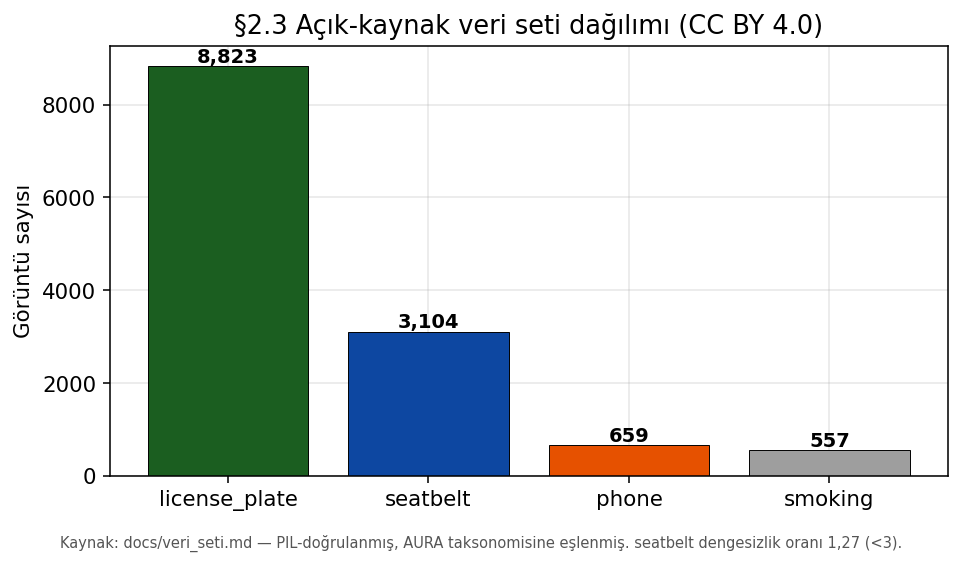
\includegraphics[width=0.43\textwidth]{fig_veri_dengesi.png}
\caption{Toplanan açık-kaynak veri setlerinin görüntü dağılımı (tümü CC BY 4.0).}
\label{fig:denge}
\end{figure}

\subsection{Veri Artırma (Augmentation)}
Augmentasyon, Ultralytics eğitim hattının yerleşik teknikleriyle uygulanır: \textbf{mozaik}
(bağlam çeşitliliği ve küçük nesne öğrenimi), \textbf{yatay flip} (yön bağımsızlığı), \textbf{HSV
jitter} (ışık/renk sıcaklığı), \textbf{karartma/gamma} (gece ve far-patlaması senaryoları) ve
\textbf{motion blur} (yüksek hızlı araç bulanıklığı). Ablasyon için \tcode{--no-augment} ile
kapatılabilir. Ek olarak, karanlık kabin görüntülerinde sürücü ROI'sine çalışma anında CLAHE+gamma
parlatma uygulanır.

\subsection{Train / Val / Test Dağılımı}
Veri varsayılan olarak \textbf{\%80 train / \%10 val / \%10 test} oranında bölünür (seed 42;
Şekil~\ref{fig:split}). Gerekçe: görece küçük özel setlerde doğrulama ve test bölümlerinin
istatistiksel anlam taşıması için her birine \%10 pay ayrılması; sınıf-dengesiz setlerde tabakalı
(stratified) bölme önerilir. Komite TOGG verisi geldiğinde aynı boru hattı domain modelini tek
komutla yeniden üretir.

\begin{figure}[ht]\centering
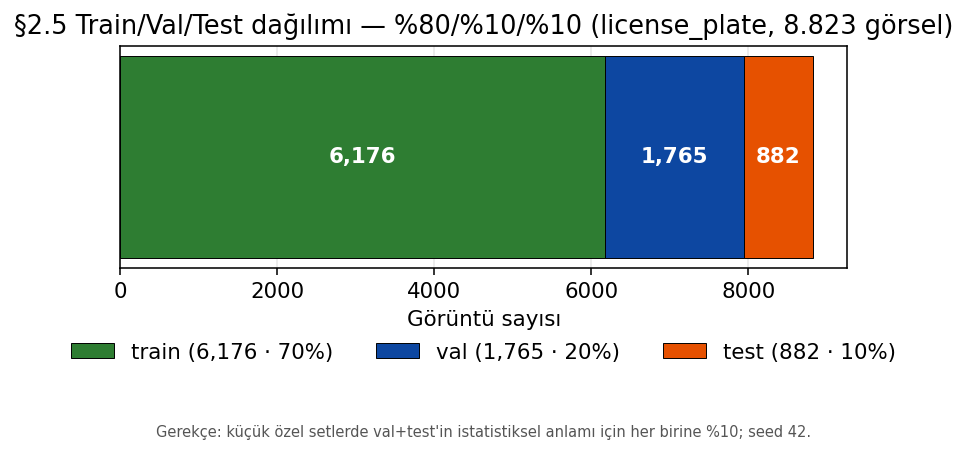
\includegraphics[width=0.45\textwidth]{fig_split.png}
\caption{\tcode{license\_plate} setinin \%80/\%10/\%10 train/val/test dağılımı (8.823 görsel).}
\label{fig:split}
\end{figure}

% ========================== 3. YZ ÇÖZÜMÜ ==============================
\section{Yapay Zekâ Çözümü}

\subsection{Problemin Analizi}
Trafik kamerası görüntüsünden tespit, kontrollü laboratuvar koşullarından farklı yapısal zorluklar
içerir. AURA, bu zorlukları gerçek footage üzerinde ölçerek tanımlamış ve her birine hedefli bir
tasarım kararıyla yanıt vermiştir (Tablo~\ref{tab:problem}). Bu problemlerin ortak noktası, kamera
gürültüsünün ve değişken görüş koşullarının kare-bazlı kararları kararsız kılmasıdır; bu nedenle
AURA'nın temel tercihi \textbf{kare-merkezli değil ID-merkezli} karar üretmektir — her araç bir
takip kimliği (\tcode{track\_id}) altında izlenir ve tüm kararlar bu kimlik üzerinde zaman içinde
biriktirilerek istikrara kavuşturulur.

\begin{table}[H]\centering\small
\caption{Temel problemler ve izlenen çözüm yolları.}\label{tab:problem}
\begin{tabularx}{\textwidth}{>{\raggedright\arraybackslash}p{4.1cm} >{\raggedright\arraybackslash}X}
\toprule
\textbf{Problem} & \textbf{İzlenen çözüm} \\ \midrule
Karanlık kabin (cam-ardı sürücü) & ROI'de CLAHE + gamma parlatma \\
Araç tipi titremesi (car$\leftrightarrow$truck) & Alan-ağırlıklı, track-bazlı sınıf oylaması \\
Hayalet (phantom) track'ler & \tcode{min\_track\_frames} çıktı kapısı + IoU dedup \\
Işık değişimi / hareket bulanıklığı & Augmentasyon (gece/gamma, motion-blur) + sürücü-ROI CLAHE/gamma parlatma \\
Oklüzyon & ID-merkezli birikim (kısa kayıpta kimlik korunur) \\
Karanlık plaka il-kodu hatası (3$\rightarrow$0/2) & Pozisyon-veto + zemin koşulu $\rightarrow$ yanlış onay yerine \tcode{pending} \\
Tek-kare yanlış-pozitif (flicker) & ID-merkezli 16/8 zaman-oylaması \\
\bottomrule
\end{tabularx}
\end{table}

\subsection{Çözüm Mimarisi}
Sistem, ham video akışını etiketli olay/annotation çıktısına dönüştüren bir \textbf{kaskad boru
hattıdır} (Şekil~\ref{fig:mimari}). Ham kare önce ön-işlemeden geçer; Aşama~1 dedektörü (YOLO26 +
ByteTrack + alan-ağırlıklı sınıf oyu) araçları tespit/takip eder ve yalnızca \textbf{iki ROI}
üretir: sürücü kabini ve plaka bölgesi. Bu ROI'ler paralel iki Aşama~2 motoruna gider — sürücü
davranışı motoru (Katman~A model + Katman~B per-ID zaman-oylaması) ve plaka okuma konsensüs döngüsü.
Hız/swerving kestirimi ID-merkezli birikim katmanını besler; nihai çıktı olay/annotation akışı
olarak dashboard, mobil ve JSONL kanıt izine yayılır. QoD tetikleri (yaklaşma, kalite, anomali) bu
akıştan türetilir. (Gerçek$\leftrightarrow$mock sınırı Bölüm 1'de tanımlanmıştır.)

\begin{figure}[H]\centering
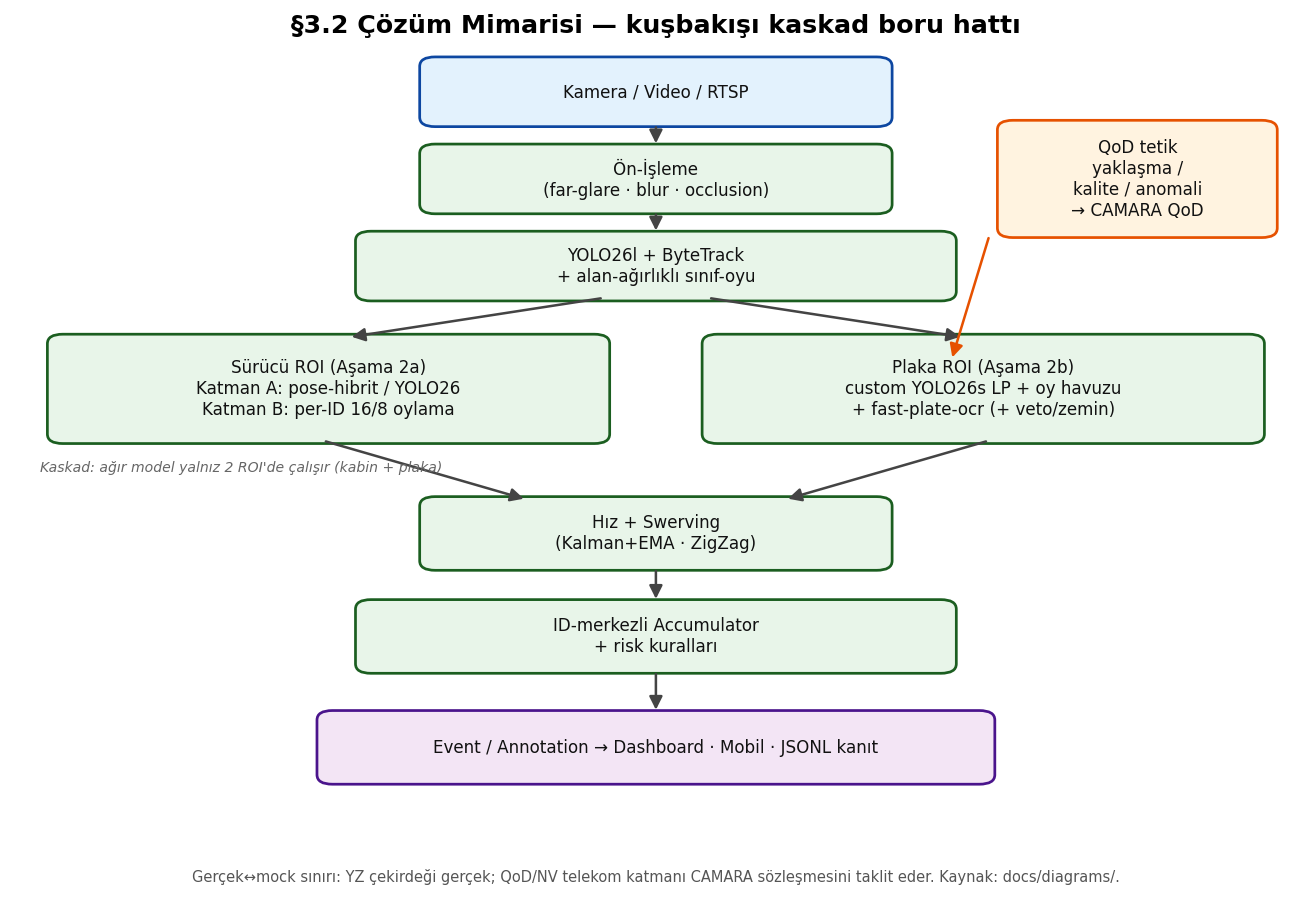
\includegraphics[width=0.96\textwidth]{fig_mimari.png}
\caption{AURA kuşbakışı kaskad boru hattı (soldan sağa akış): Aşama-1 tespit/takipten iki ROI ile üç paralel Aşama-2 motoruna (sürücü davranışı $\parallel$ plaka okuma $\parallel$ hız) ve ID-merkezli birikime; QoD tetikleyici (kesikli) kritik anda 5G kalitesini talep eder.}
\label{fig:mimari}
\end{figure}

\subsection{Çözüm Detayları}
\textbf{Ön-işleme.} Ön-işleme katmanı far-patlaması, motion-blur, yansıma ve occlusion için
config'ten aç/kapanabilen filtre kancaları sunar; mevcut sürümde fiilen uygulanan iyileştirme,
OCR ve sürücü-durumu doğruluğunu artıran \textbf{ROI-düzeyi} işlemedir: plaka/sürücü kırpığına
CLAHE + gamma parlatma ve küçük kırpık için süper-çözünürlük (gece/loş koşul telafisi).

\textbf{Aşama 1 — Tespit ve Takip.} Ana dedektör varsayılan olarak doğruluk-önce stok \tcode{yolo26l}
(Ultralytics 8.4, en güncel YOLO ailesi); \tcode{ByteTrack} her araca benzersiz kimlik atar. Aynı
aracın kareler arası sınıf salınımı (uzaktan \tcode{truck}, yakından \tcode{car}), track başına
\textbf{alan-ağırlıklı sınıf oylaması} (\tcode{güven $\times$ bbox\_alan/kare\_alan}) ile çözülür.

\textbf{Aşama 2a — Sürücü Davranışı (iki katman).} Sürücü ROI'si önce kişi kutusuna daraltılır.
Katman~A iki backend'den birini kullanır: fine-tune YOLO26 detection veya — fine-tune gerektirmeyen —
\textbf{YOLO26-pose} keypoint geometrisi (bilek$\leftrightarrow$ağız/kulak göreli yakınlığı,
yüz-genişliği biriminde, ölçek-bağımsız), nesne kanıtıyla hibrit güçlendirilir; landmark/MediaPipe
kütüphanesi \textbf{kullanılmaz}. Katman~B (\tcode{DriverStateEngine}) her track için zaman-oylaması
yürütür: bir bayrak son 16 karenin en az 8'inde doğruysa aktif sayılır (tek-kare yanlış-pozitif elenir).

\textbf{Aşama 2b — Plaka Okuma ve Konsensüs.} Araç sweet-spot'a girince OCR etkinleşir; \textbf{özel
eğitimli YOLO26s LP dedektörü} (\tcode{custom\_license\_plate}, held-out mAP50 0,983) plakayı sıkı
kırpar. Plakaya-özel hafif ONNX motoru \textbf{fast-plate-ocr} (varsayılan; kurulu değilse
\tcode{EasyOCR} fallback) okur. Her okuma, OCR güveni $\times$ kaynak kalitesi (LP kırpık yüksekliği)
ile ağırlıklanıp track ömrü boyunca \textbf{kalıcı oy havuzunda} biriktirilir. Türk plaka formatına
(\tcode{\^{}\textbackslash d\{2\}[A-Z]\{1,3\}\textbackslash d\{2,4\}\$}) normalize edilen okumalar
pozisyon-hizalı karakter füzyonuyla birleştirilir; onay için her pozisyonda kazanan karakter ikinciyi
mutlak bir marjla geçmek zorundadır, aksi halde karar \tcode{pending}'e çevrilir — sistem
\textbf{belirsiz okumayı tasarım gereği onaylamaz}.

\textbf{Stabilite/Doğruluk Zırhları (K-004, config-driven).} (i) Kayan-karakter onay marjı
(\tcode{confirm\_min\_char\_margin=2.0}): pozisyon belirsizse plaka onaylanmaz, \tcode{pending} denir.
(ii) Takip/phantom çıktı kapısı (\tcode{track\_id=-1}, \tcode{min\_output\_frames}): kimliğe bağlanmamış
hayalet tespitler olay üretmez. (iii) ROI alan tavanı (\tcode{max\_roi\_area\_ratio=0.10}): anormal
büyük ROI'ler kırpılır. Hiçbir eşik videoya-özel sabit içermez (oran-bazlı, ölçek-bağımsız).

\textbf{Hız ve Swerving.} Hız kalibrasyon-bağımlıdır (tripwire/ipm/metric, Kalman+EMA); kalibrasyon
yoksa sistem mutlak hız iddia etmez, yalnız göreli-hız bayrağı üretir. Swerving, aracın merkez-x
serisindeki ZigZag ekstremum sayımıyla (araç-genişliği birimi, saniye penceresi) kalibrasyonsuz tespit
edilir.

\textbf{Yazılım ve Donanım.} Python 3.13, PyTorch (Ultralytics 8.4.66), fast-plate-ocr/EasyOCR,
OpenCV, Shapely, FastAPI/Uvicorn. Cihaz otomatik seçilir (CUDA $\rightarrow$ MPS $\rightarrow$ CPU).
Geliştirme Apple Silicon/MPS; hedef sunucu dağıtımı NVIDIA CUDA üzerindedir — gerçek ölçüm donanımı
RTX 5070 Laptop GPU (4.608 CUDA çekirdeği, 8 GB VRAM, Compute 12.0/Blackwell, torch 2.8.0+cu128;
bkz. Bölüm 4.6).

% ========================== 4. SINAMA ================================
\section{Çözümün Sınanması}

\subsection{Sınama Protokolü}
Çözüm üç tamamlayıcı düzeyde sınanmıştır: (i) etiketli \textbf{held-out doğrulama setleri} üzerinde
istatistiksel tespit doğruluğu (mAP/P/R; Bölüm 4.2); (ii) üç gerçek test videosu (kapalı otopark, TOGG;
GT plaka \tcode{34TC8532}) üzerinde davranış P/R/F1, plaka exact-match (CER ile), FPS (Bölüm 4.3--4.6);
(iii) QoD'nin başarım katkısı (A/B), kare-düzeyi GT içeren kontrollü sentetik set üzerinde (Bölüm 4.5).
Şartnamenin 4.5 maddesi gereği (``kanıtlanamayan hedef puanlanmaz''), rapordaki her sayı bir komuta ve
artefakta bağlıdır (Bölüm 4.7).

\subsection{Tespit Doğruluğu (held-out mAP / P / R / F1)}
Özel sınıfların YOLO26s fine-tune eğitimi \textbf{tamamlanmıştır}; ayrılmış test bölmesinde ölçülen
held-out doğrulukları Tablo~\ref{tab:map} ile Şekil~\ref{fig:map}'de verilmiştir.
Varsayılan stok \tcode{yolo26l} ayrıca COCO val2017 (5.000 görsel) held-out üzerinde değerlendirilmiştir
(genel doğruluk göstergesi). Telefon (\tcode{phone}) tespiti stok \tcode{yolo26l}'in COCO ``cell phone''
sınıfıyla yapılır; ayrı özel held-out ölçümü yoktur (davranış doğruluğu Tablo~\ref{tab:beh}'de
video-düzeyinde verilmiştir).

\begin{table}[H]\centering\small
\caption{Held-out tespit doğruluğu (özel modeller ayrılmış test bölmesinde; stok \tcode{yolo26l} COCO val2017'de). \tcode{license\_plate} üretimde varsayılan LP dedektörüdür. $^{\dagger}$\,\tcode{seatbelt}/\tcode{smoking}: fine-tune held-out sonuçları (üretim hattında opsiyonel/devre-dışı).}\label{tab:map}
\begin{tabularx}{\textwidth}{>{\raggedright\arraybackslash}X cccccc}
\toprule
\textbf{Model / set} & \textbf{mAP50} & \textbf{mAP50-95} & \textbf{Precision} & \textbf{Recall} & \textbf{F1} \\ \midrule
\tcode{license\_plate} (\tcode{yolo26s}) & \textbf{0,983} & 0,706 & 0,982 & 0,963 & 0,973 \\
\tcode{seatbelt} (\tcode{yolo26s})$^{\dagger}$ & 0,895 & 0,546 & 0,844 & 0,795 & 0,818 \\
\tcode{smoking} (\tcode{yolo26s})$^{\dagger}$ & 0,856 & 0,457 & 0,855 & 0,820 & 0,837 \\
\tcode{yolo26l} — COCO val2017 (genel) & 0,709 & 0,537 & 0,740 & 0,641 & -- \\
\bottomrule
\end{tabularx}
\end{table}

\begin{figure}[ht]\centering
\begin{minipage}{0.46\textwidth}\centering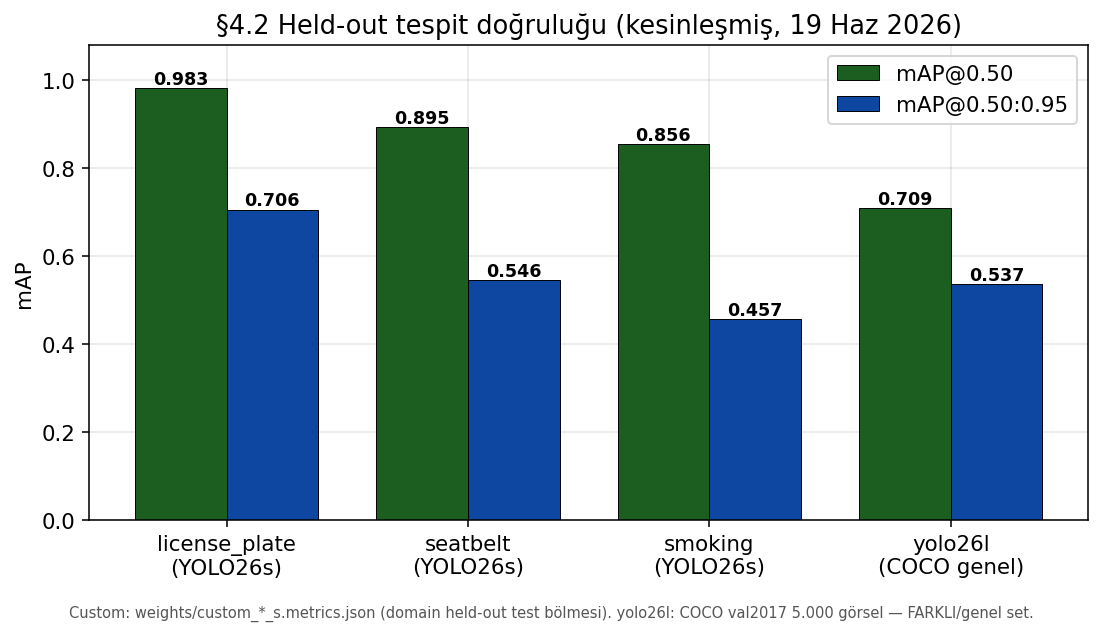
\includegraphics[width=\textwidth]{fig_tespit_map.png}\end{minipage}\hfill
\begin{minipage}{0.46\textwidth}\centering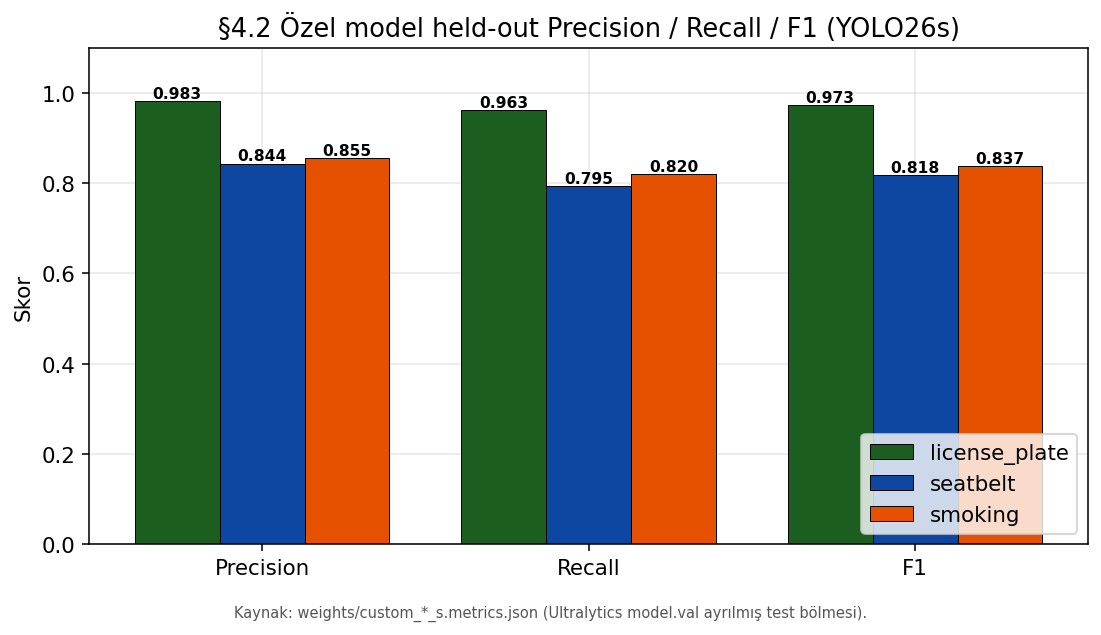
\includegraphics[width=\textwidth]{fig_custom_prf1.png}\end{minipage}
\caption{Sol: held-out mAP50 / mAP50-95. Sağ: özel modellerin held-out Precision / Recall / F1 (\tcode{yolo26s}). Stok \tcode{yolo26l} COCO genel settir.}
\label{fig:map}
\end{figure}

\subsection{Davranış Tespiti (P / R / F1)}
Üç gerçek video üzerinde video-düzeyi davranış tespiti iki dedektör profiliyle ölçülmüştür
(Tablo~\ref{tab:beh}). \textbf{Her iki dedektör de} çapraz yanlış-pozitif üretmez (makro-F1 1,0;
\tcode{phone}/\tcode{smoking}/\tcode{swerving} için P=R=F1=1,0); araç sınıfı doğruluğu (accuracy)
\textbf{\%100}'dür. \textit{Kapsam ve sınırlılık:} sınıf başına destek N=1;
held-out istatistiksel güç yalnız \tcode{smoking}'i (mAP 0,856; Tablo~\ref{tab:map}) doğrudan
destekler --- \tcode{phone} stok-COCO ``cell phone'' sınıfıyla, \tcode{swerving} kalibrasyonsuz
geometriyle tespit edilir; bu ikisi için held-out sınıf metriği yoktur, video sonucu uçtan-uca
varlık-kanıtıdır. Emniyet kemeri (\tcode{seatbelt}) yalnızca held-out mAP (0,895) ile sınanmıştır; üç
videoda kemer-GT örneği bulunmadığından video-düzeyi P/R/F1 raporlanmamıştır.

\begin{table}[H]\centering\small
\caption{Davranış tespiti — üç gerçek test videosunda video-senaryo düzeyi sonuç (her hücre P/R/F1). \textbf{Aşama-1 profili} yalnız ana dedektörü değiştirir; \tcode{phone} stok COCO ``cell phone'' nesne-kanıtıyla, \tcode{smoking} hand-to-mouth poz-geometrisiyle (COCO'da sigara sınıfı yoktur; \tcode{v4} satırında özel model de etkin), \tcode{swerving} dedektörden bağımsız kinematikle üretilir.}\label{tab:beh}
\begin{tabularx}{\textwidth}{>{\raggedright\arraybackslash}X cccc}
\toprule
\textbf{Aşama-1 profili} & \textbf{phone} & \textbf{smoking} & \textbf{swerving} & \textbf{Makro F1} \\ \midrule
\tcode{yolo26l} (stok, varsayılan) & 1,0/1,0/1,0 & 1,0/1,0/1,0 & 1,0/1,0/1,0 & \textbf{1,00} \\
\tcode{v4-finetune} (A/B kıyas tabanı) & 1,0/1,0/1,0 & 1,0/1,0/1,0 & 1,0/1,0/1,0 & \textbf{1,00} \\
\bottomrule
\end{tabularx}
\end{table}

\subsection{Plaka Okuma — A/B}
Karanlık otopark koşulları, plaka okumayı en kritik doğrulama sınaması yapar. Baseline OCR (EasyOCR)
ile üretim hattının (özel YOLO26s LP + fast-plate-ocr) A/B'si Tablo~\ref{tab:plate}'tedir:
fast-plate-ocr, baseline'ın \tcode{video\_3}'teki sistematik il-kodu
misread'ini (\tcode{24IC8532}) düzelterek sonucu \textbf{3/3 tam-eşleşme, CER 0,0}'a çekmiş,
\tcode{video\_1}/\tcode{video\_2}'yi korumuştur; her iki hatta da \textbf{yanlış-onay sıfırdır}.

\begin{table}[H]\centering\small
\caption{Plaka okuma A/B — 3 gerçek test videosu, gerçek-değer (GT) plaka \tcode{34TC8532}.}\label{tab:plate}
\begin{tabularx}{\textwidth}{>{\raggedright\arraybackslash}X ccccc}
\toprule
\textbf{Hat} & \textbf{Exact-match} & \textbf{CER} & \textbf{Confirmed} & \textbf{Partial} & \textbf{Yanlış-onay} \\ \midrule
Baseline (EasyOCR · stok/v4) & 2/3 (\%66,7) & 0,083 & 2 & 1 & \textbf{0} \\
\textbf{Production} (custom\_LP + fast-plate-ocr) & \textbf{3/3 (\%100)} & \textbf{0,0} & 3 & 0 & \textbf{0} \\
\bottomrule
\end{tabularx}
\end{table}


En kritik tasarım garantisi: sistem belirsiz/uzak/bulanık bir okumayı \textbf{kesinleştirmemek üzere
tasarlanmıştır} (üç videoda yanlış-onay görülmemiştir); yakın-net video doğru plakayı CONFIRMED
verirken belirsiz okuma \tcode{pending}'te kalır. Bu davranış Bölüm 3.3'teki onay marjı, pozisyon-veto ve zemin koşulu zırhlarının
ölçülen sonucudur.

\subsection{QoD Entegrasyonu ve Talep-Yönlü Kaynak Verimliliği}
QoD'nin temel değeri her kareyi yüksek kalitede taşımak değil, sistemi düşük-bant genel izleme modunda
çalıştırıp \textbf{yalnızca kritik anda} (yaklaşan araç, küçük/uzak plaka) 5G yüksek-kalite talep
etmektir — yani \textbf{talep-yönlü kaynak verimliliği}. \tcode{vehicle\_approach} tetiği şartnamenin
``TOGG yaklaşınca QoD'' senaryosunu birebir karşılar.

Katkı, A/B harness ile yeniden-üretilebilir biçimde ölçülür (aynı kaynak QoD OFF/ON ile koşulur).
\textbf{Ölçüm sınırı:} mevcut kontrollü koşuda OFF baseline'ı zaten yeterli kalitede olduğundan
doğruluk-deltası $\approx$0'dır; pozitif delta yalnızca OFF bant/çözünürlük baskısı altında (küçük/uzak
plaka ROI'si okunamaz piksele düştüğünde) beklenir. \textbf{Mevcut koşuda QoD bir doğruluk artışı
göstermemiştir}; bu nedenle QoD katkısı bu raporda doğruluk iyileşmesi olarak değil, CAMARA sözleşmesine
uyumlu \textbf{talep-yönlü tetikleme ve kaynak verimliliği} olarak sunulur. Üç-kollu A/B (Always-LOW /
Always-HIGH / Adaptive-QoD) baskılı sette doğruluk-deltasını ve bant tasarrufunu ölçmeye hazırdır.

\subsection{İşleme Hızı (FPS)}
İşleme hızı hem geliştirme ortamında (Apple Silicon/MPS, M4 Pro) hem de hedef sunucu donanımında
(NVIDIA RTX 5070 Laptop GPU, \textbf{4.608 CUDA çekirdeği}) \textbf{gerçek ölçümle} değerlendirilmiştir
(Tablo~\ref{tab:fps}; her profilde 100+ kare ölçümü, 26.06.2026). CUDA,
MPS geliştirme alt-sınırının (\tcode{yolo26l} $\sim$5,9 FPS) \textbf{${\approx}2\times$}'i iş-hacmi sağlar.

\begin{table}[H]\centering\small
\caption{İşleme hızı — gerçek ölçüm: CUDA (RTX 5070 Laptop GPU) ve MPS (M4 Pro); 26.06.2026.}\label{tab:fps}
\begin{tabularx}{\textwidth}{>{\raggedright\arraybackslash}X ccc}
\toprule
\textbf{Profil · dedektör · imgsz} & \textbf{Ortalama FPS} & \textbf{p50 (ms)} & \textbf{p95 (ms)} \\ \midrule
\tcode{server} · \tcode{yolo26l} · 960 (CUDA) & \textbf{12,31} & 80 & 93 \\
\tcode{laptop} · \tcode{yolo26s} · 640 (CUDA) & \textbf{14,72} & 65 & 88 \\
\tcode{server} · \tcode{yolo26l} (MPS, M4 Pro) & $\sim$5,9 & -- & -- \\
\bottomrule
\end{tabularx}
\end{table}

Kare-başına \textbf{gecikme} (p95=93 ms) ile \textbf{iş-hacmi} (${\sim}$12 FPS) ayrı büyüklüklerdir.
Bu rakam \textbf{tüm hattın} (Aşama-1 + Aşama-2) değeridir; zaman-kritik olan \textbf{Aşama-1 tespit/takip}
her karede ve daha yüksek hızda çalışır, pahalı Aşama-2 (OCR/poz) ise yalnız ROI'lerde ve olay-tetiğiyle
koşar. Dolayısıyla kare-örnekleme takip sürekliliğini değil, yalnızca Aşama-2 yoğunluğunu seyreltir;
sistem ${\sim}$12 FPS iş-hacmiyle 25--30 FPS'lik akışı olay-tespiti amacıyla işler ve p95 gecikme zarfı
bu kullanım için yeterlidir.


\subsection{Hız, Kanıt İzi ve Güven Dayanakları}
\textbf{Hız/swerving.} Metrik hız modülü (IPM/homografi + Kalman) uygulanmıştır ve sahne kalibrasyonu
sağlandığında MAE/MAPE üretir; bu raporda mutlak hız MAE/MAPE \textbf{kapsam dışıdır} (sahne
kalibrasyonu gerektirir, finalde mekândan sağlanır). Kalibrasyon gerektirmeden çalışan ve bu raporda
sınanan yetenek swerving'dir: üç videodan \tcode{video\_3}'te tespit edilmiş ve davranış makro-F1'ine
dahildir (Bölüm 4.3).

\textbf{Kanıt izi ve izlenebilirlik (şartname 4.5).} Rapordaki sayılar elle değil, otomatik bir
ölçüm hattıyla üretilmiştir: sistem her işlemede (1) zaman-damgalı olay izi (JSONL), (2) annotated
video ve (3) karar/oy dökümü çıkarır; bir metrik-raporlama aracı Bölüm~4 tablolarını bu çıktılardan
toplar. Böylece her sayı izlenebilir bir ölçüme dayanır, rapora elle girilmemiştir. Otomatik test
paketinin (${\sim}780$ test) bir bölümü ayrıca CAMARA QoD/NV mock sözleşme uyumunu doğrular.

\textbf{Güven dayanakları.} Güven, ölçülen sayıların ötesinde \textbf{yapısal} gerekçelere
dayanır: tüm eşikler oran/boyut-temelli ve ölçek-bağımsızdır (videoya-özel sabit yok, K-004), dolayısıyla
sonuçlar tek çekime aşırı-uyumlanmaz; belirsizlikte sistem yanlış üretmek yerine çekimser kalır
(plakada \textbf{sıfır yanlış-onay}) ve bu güvenceler config-driven, gerçek videoda doğrulanmış zırhlara
(Bölüm 3.3) dayanır. Video setinin istatistiksel sınırı (N=1) Bölüm~4.3'te açıkça belirtilmiş olup
komite verisiyle güçlendirilecektir.

% ========================== 5. KAYNAKÇA ==============================
\section{Kaynakça}
{\footnotesize Aşağıda projede fiilen kullanılan başlıca yöntem, kütüphane ve açık-veri kaynakları (lisanslarıyla) listelenmiştir.\par}
\footnotesize\sloppy
\begin{enumerate}\setlength{\itemsep}{0pt}\setlength{\parskip}{0pt}
\item Ultralytics, \textit{Ultralytics YOLO Documentation} (v8.4.66, YOLO26), 2026. \url{https://docs.ultralytics.com} (erişim 2026).
\item Y. Zhang vd., \textit{ByteTrack: Multi-Object Tracking by Associating Every Detection Box}, ECCV, 2022. arXiv:2110.06864.
\item T.-Y. Lin vd., \textit{Microsoft COCO: Common Objects in Context}, ECCV, 2014. arXiv:1405.0312. (CC BY 4.0)
\item ankandrew, \textit{fast-plate-ocr}, 2024--2026. \url{https://github.com/ankandrew/fast-plate-ocr}.
\item JaidedAI, \textit{EasyOCR}, 2020--2026. \url{https://github.com/JaidedAI/EasyOCR}. (Apache-2.0)
\item K. Zuiderveld, \textit{Contrast Limited Adaptive Histogram Equalization (CLAHE)}, Graphics Gems IV, 1994 · R. E. Kalman, \textit{A New Approach to Linear Filtering}, ASME J. Basic Eng., 1960. (ön-işleme / hız)
\item CAMARA Project (Linux Foundation), \textit{Quality-on-Demand API} \& \textit{Number Verification API}, 2023--2026. \url{https://github.com/camaraproject}.
\item 3GPP, \textit{System Architecture for the 5G System}, TS 23.501, Rel-18. \url{https://www.3gpp.org}.
\item keremberke, \textit{License Plate Object Detection}, Hugging Face, 2023. (CC BY 4.0) --- \tcode{license\_plate} 8.823 görsel.
\item ramankamran, \textit{Seatbelt Detection (YOLOv11)}, Hugging Face, 2024. (CC BY 4.0) --- \tcode{seatbelt} 3.104 görsel.
\item \textit{CigDet — Cigarette Detection}, Mendeley Data, 2021. DOI:10.17632/6hyrr8typ7.1. (CC BY 4.0) --- \tcode{smoking} 557 görsel.
\item anywaylabs, \textit{Synthetic Driver Monitoring}, Hugging Face, 2024. (CC BY 4.0) --- \tcode{phone} 659 görsel.
\item M. Everingham vd., \textit{The PASCAL VOC Challenge} (mAP metodolojisi), IJCV, 2010.
\end{enumerate}
{\footnotesize\textit{Yapay zekâ desteği:} raporun yazım/düzenlenmesinde büyük dil modeli araçlarından yararlanılmıştır; tüm teknik içerik, ölçüm ve sayılar takımca üretilip doğrulanmıştır.\par}
\normalsize

\end{document}
